%!TeX program = xelatex
\documentclass[12pt,hyperref,a4paper,UTF8]{ctexart}
\usepackage{SJTUReport}
\usepackage{graphicx}
\usepackage{subfigure}
\usepackage{parskip}
%%-------------------------------正文开始---------------------------%%
\begin{document}

%%-----------------------封面--------------------%%
\cover

%%------------------摘要-------------%%
%\begin{abstract}
%
%在此填写摘要内容
%
%\end{abstract}

\thispagestyle{empty} % 首页不显示页码

%%--------------------------目录页------------------------%%
\newpage
\tableofcontents

%%------------------------正文页从这里开始-------------------%
\newpage

%%可选择这里也放一个标题
%\begin{center}
%    \title{ \Huge \textbf{{标题}}}
%\end{center}

\section{实验目的}
\begin{itemize}
    \item 了解化学振荡反应的基本原理。
    \item 掌握化学振荡反应的电势测定方法与表观活化能。
    \item 初步理解自然界中普遍存在的平衡非线性问题。
    \item 用电动势法测定甲酸被溴氧化的反应动力学方程。
    \item 加深对于反应速率方程,反应级数等概念的认识。
\end{itemize}

\section{实验原理}
\subsection{BZ振荡反应}
\subsubsection{基本情况}
通常情况下,化学反应体系的反应物浓度随反应时间呈单调变化直至平衡状态。但是,在某些反应体系中部分反应物浓度随时间成周期性变化,这一现象成为化学振荡。最著名的化学振荡反应为BZ振荡反应,指可呈现化学振荡现象的含溴酸盐的反应体系。大量实验表明,发生化学振荡的体系必须远离平衡态,且反应中含有自催化步骤,体系同时具有双稳定态,故体系可在两种稳定态中来回振荡。

\subsubsection{反应解释}
1972年,费尔特(Field),寇罗斯(Koros)和诺伊斯(Noyes)等人通过实验对BZ振荡反应作出了解释。对于著名的化学振荡反应

\ce{ 2BrO3^{-} + 3CH2(COOH)_2 + 2H^{+} ->[Ce^{3+},Br^{-}]2BrCH(COOH)_2 +3CO_2 + 4H2O}

FKN机理认为在硫酸介质中,以铈离子为催化剂时丙二酸被溴酸盐氧化的过程可分为几种情况:
\begin{enumerate}
    \item 当$Br^-$浓度足够高时,$BrO_3^-$通过下列反应被还原为$Br_2$。
    \begin{enumerate}
        \item \ce{ BrO3^{-} + 2Br^{-} + 2H^{+} -> HBrO_2 + HBrO}
        \item \ce{ HBrO_2 + Br^{-} + H^{+} -> 2HBrO}
        \item \ce{ 2HBrO + Br^{-} + H^{+} -> Br_2 + H_2O}
    \end{enumerate}

    其中反应(a)为控速步骤,上述反应产生的$Br_2$使丙二酸溴化,其反应为

    \ce{ Br2 + CH2(COOH)_2 -> BrCH(COOH)_2 + Br^{-} + H^{+} }

    总反应为上述4个反应的总和
    
    \textbf{\ce{Br2 + 2Br^{-} + 3H^{+} + 3CH2(COOH)_2 -> 3BrCH(COOH)_2 + 3H_2O}} (1)
    
    \item 当$Br^{-}$浓度较低时,$Ce^{3+}$通过下列反应被氧化。
    \begin{enumerate}
        \item \ce{2HBrO_2 -> BrO3^{-} + HBrO + H^{+}}
        \item \ce{ HBrO2 + BrO3^{-} + H^{+} -> 2BrO_2 + H_2O}
        \item \ce{ Ce^{3+} + BrO_2 + H^{+} -> HBrO_2 + Ce^{4+}}
    \end{enumerate}

    其中反应(b)是速率控制步骤,上述反应总反应为

    \textbf{\ce{ 2BrO3^{-} +4Ce^{3+} + 5H^{+} -> HBrO + 4Ce^{4+} + 2H_2O}} (2)

该反应是振荡反应得以发生必需的自催化反应。自催化反应是振荡反应不可缺少的步骤,否则振荡不能发生。
\end{enumerate}

最后,$Br^{-}$通过下面反应再生

\textbf{\ce{ 2BrCH(COOH)_2 +4Ce^{4+} + 2H2O -> Br- + HCOOH + 4Ce^{3+} + 2CO2 + 5H+}}

\textbf{\ce{ HCOOH + HBrO -> Br- + CO2 + H2O + H+}}

**上述两反应的总反应为
\ce{ BrCH(COOH)2 + 4Ce^{4+} + HBrO + H2O -> 2Br- + 4Ce^{3+} + 3CO2 + 6H+} (3)

将反应(1)(2)(3)相加可组成反应体系的振荡周期,即可得到著名的化学振荡反应。过程中反应(3)较为重要,反应(3)使$Br^{-}$和$Ce^{3+}$得以再生,是反应可以重复进行,形成周期性的振荡。同时,$Br^{-}$为控制离子,其浓度大于某临界浓度时发生反应(1),小雨临界浓度时发生反应(2)。

\subsubsection{实验方法}
本实验采用电化学方法观察化学振荡现象。
\begin{figure}[htp]
    \centering
    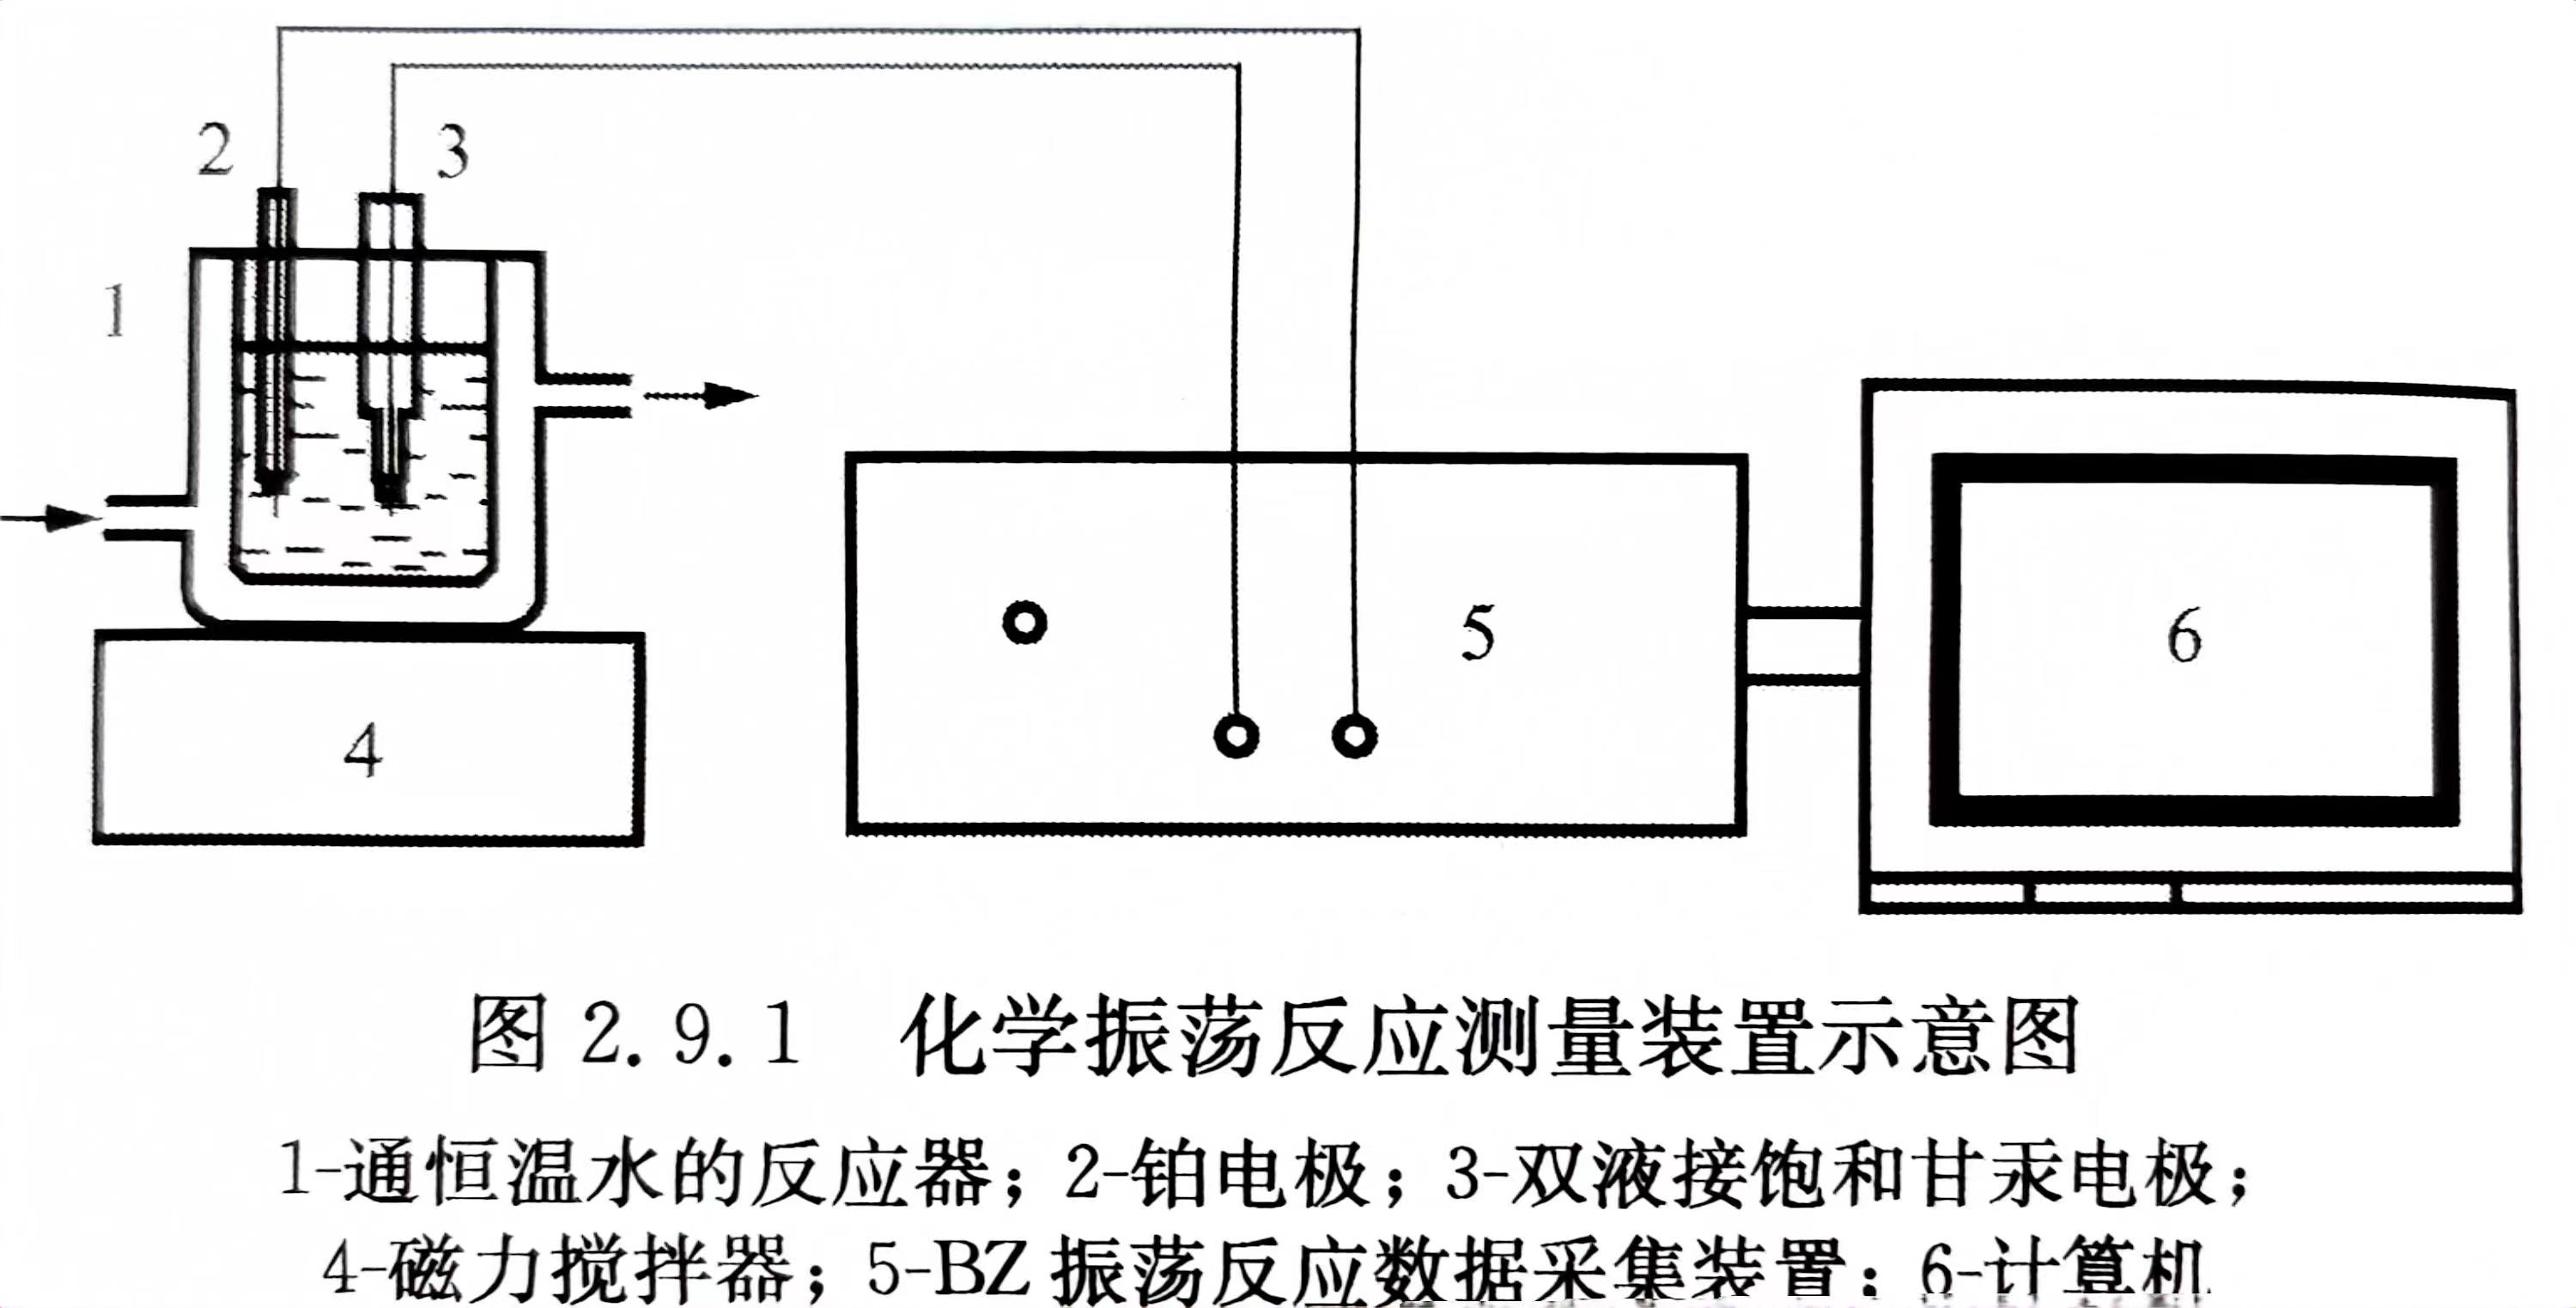
\includegraphics[width=0.6\linewidth]{1.jpg}
    \label{fig:enter-label1}
\end{figure}

以饱和甘汞电极(带盐桥)为参比电极,铂电极为导电电极,所构成的电池电动势
\begin{equation}
    E = \varphi _{\frac{Ce^{4+}}{Ce^{3+}}} - \varphi _{\text{甘汞}}
\end{equation}


通过测定不同温度下溶液中$\varphi _{\frac{Ce^{4+}}{Ce^{3+}}}$浓度比随时间的变化而产生的电势变化曲线。
\begin{figure}[htp]
    \centering
    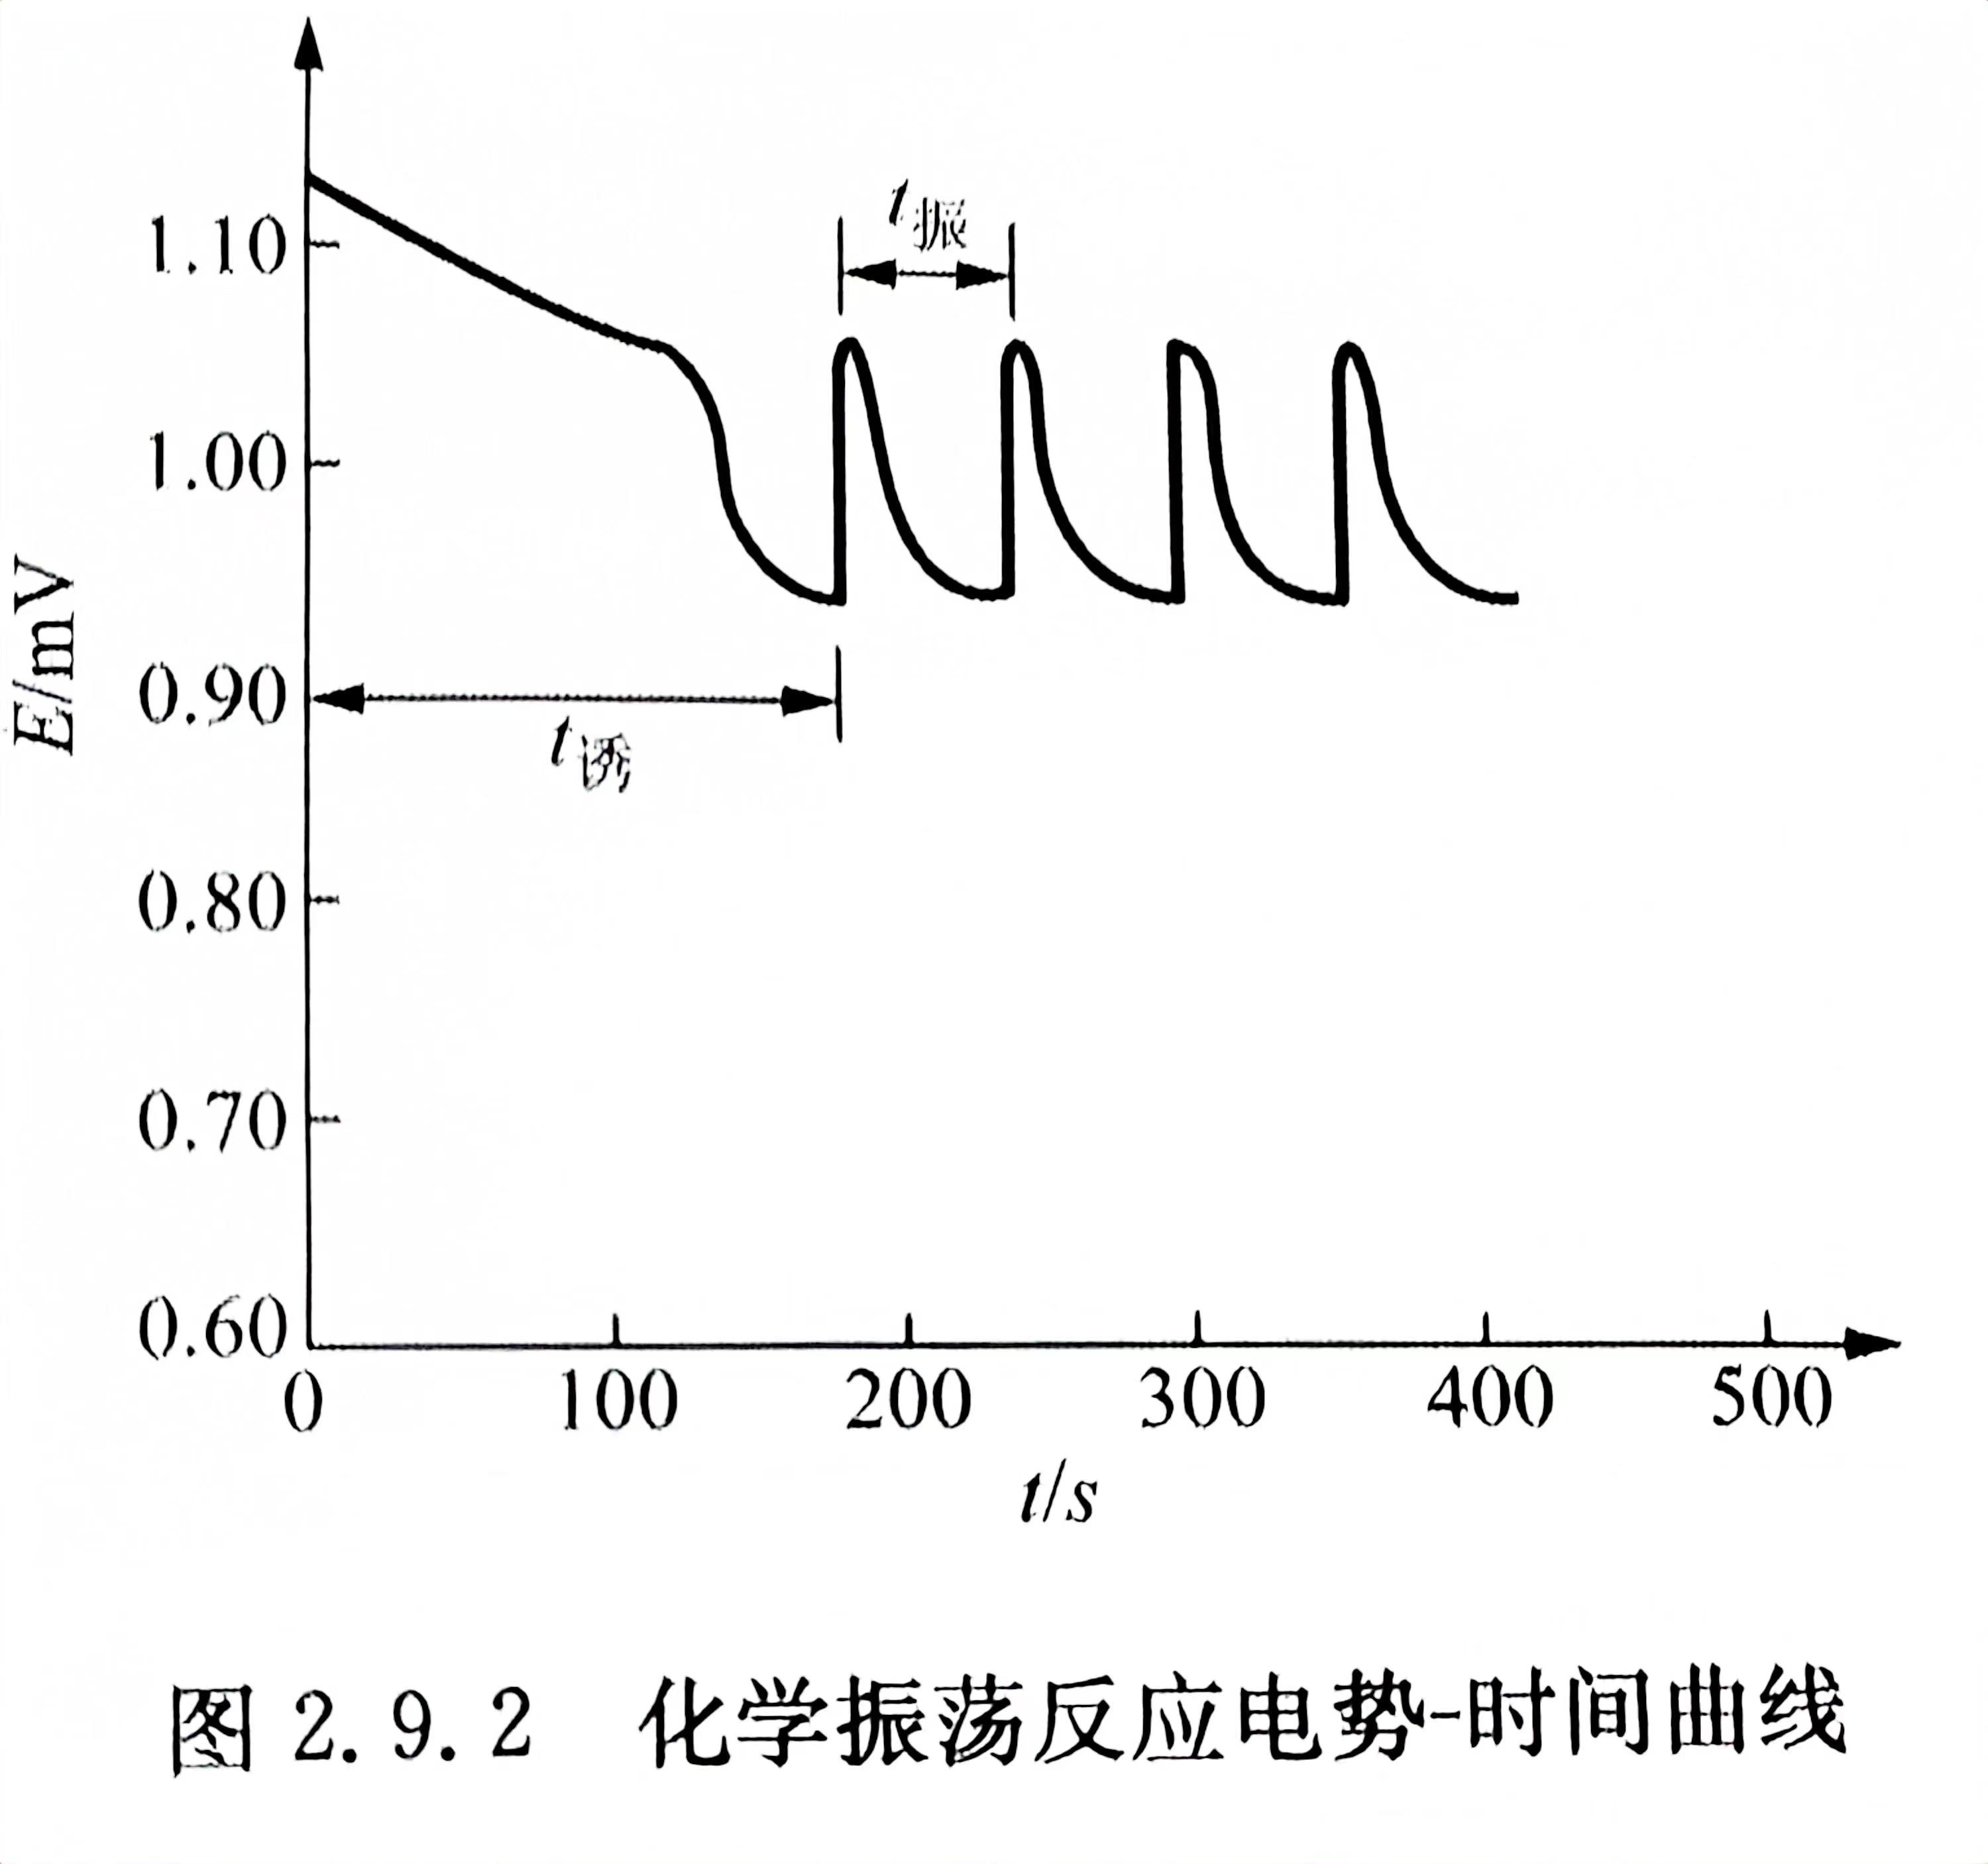
\includegraphics[width=0.6\linewidth]{2.jpg}
    \label{fig:enter-label}
\end{figure}

从曲线上可获得诱导期$t_{\text{诱}}$和振荡周期$t_{\text{振}}$,并根据关系式
\begin{equation}
    ln(\frac{1}{t}) = -\frac{E}{RT} + C
\end{equation}

通过作图,由直线斜率分别求出诱导活化能和振荡活化能。本实验诱导期可由振荡曲线上读取,或者由反应测量软件自动给出,成为起波时间。振荡周期需要从曲线上读取。

\clearpage

\subsection{甲酸氧化动力学}
\subsubsection{基本情况}
宏观化学动力学将反应速率与宏观变量浓度、温度等联系起来,建立反应速奉方程,方程包含速率常数、反应级数、活化能和指前因子等特征参数,动力学实验主要就是测定这些特征参数。本实验讨论甲酸氧化反应的动力学问题,一定条件下它是简单的一级反应。

\subsubsection{反应解释}
甲酸被溴氧化的反应的计量方程式如下:
\ce{HCOOH + Br2 -> CO2 + 2H+ + 2Br-}

对该反应来说,除反应物外$Br^{-}$和$H^{+}$对反应速率也有影响。具体实验中,当使$Br^{-}$和$H^{+}$过量,保持其浓度在反应中近似不变时,反应方程变为
\begin{equation}
    - \frac{\mathrm{d}{[Br^{-}]}}{\mathrm{d}t} = k {[HCOOH]}^{m}{[Br]}^n 
\end{equation}

又若$HCOOH$初始浓度远高于$Br_2$浓度,反应速率方程变为
\begin{equation}
    - \frac{\mathrm{d}{[Br^{-}]}}{\mathrm{d}t} = k^{'}{[Br]}^n
\end{equation}

式中$k^{'} = k {[HCOOH]}^{m}$

因此,只要实验测得$[Br_2]$随时间t变化的函数关系,即可确定反应级数n和速率系数。在同一温度下,改变HCOOH浓度,则可通过联立两个方程求得反应级数m和速率系数k。

\subsubsection{实验方法}
本实验采用电动势法跟踪$[Br_2]$随时间的变化,以饱和甘汞电极与置于$Br_2$和$Br^{-}$溶液中的铂电极组成电池,该电池电动势为
\begin{equation}
    E = \varphi _{{Br_2}/{Br^-}} + \frac{RT}{2F}ln\frac{[Br_2]}{[Br^-]}- \varphi _{\text{甘汞}}
\end{equation}

若$Br^-$很大,在反应过程中$Br^-$浓度可认为保持不变,上式可写成
\begin{equation}
    E = \frac{RT}{2F}ln{[Br_2]} + C
\end{equation}

若甲酸氧化反应对$Br_2$为一级,则
\begin{equation}
    - \frac{\mathrm{d}{[Br^{-}]}}{\mathrm{d}t} = k^{'}{[Br]}
\end{equation}

积分得
\begin{equation}
    ln[Br_2] = C- k^{'}t
\end{equation}

代入(6)式得
\begin{equation}
    E = C - \frac{RT}{2F}k^{'}t
\end{equation}

因此,若甲酸氧化反应对$Br_2$为一级反应,则E-t图像为一直线,并可通过斜率求得反应动力学方程。上述电池的电动势约为0.8V,而反应过程电动势的变化仅有30mV左右。当用自动记录仪或电子管伏特计测量电势变化时,为了提高测量精度而采用图1的接线法。图中用蓄电池或用电池串接1k欧姆绕线电位器,于其中分出一恒定电压与电池同极连接,使电池电势对消一部分。调整电位器,使对消后剩下约20~30毫伏,因而可使测量电势变化的精度大大提高。
\begin{figure}[htp]
    \centering
    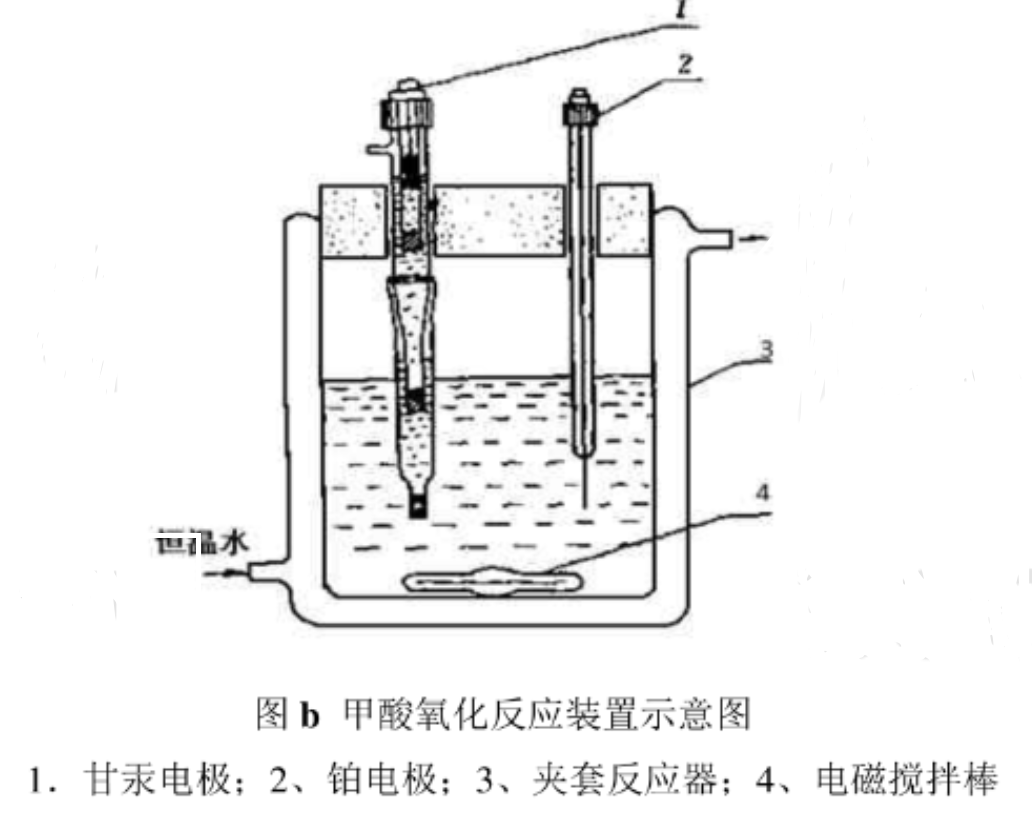
\includegraphics[width=0.5\linewidth]{3.png}
    \caption{甲酸氧化动力学装置示意图}
    \label{fig:enter-label3}
\end{figure}

\section{实验试剂与仪器}
\subsection{BZ振荡反应}
\subsubsection{实验仪器}
\begin{itemize}
    \item BZ振荡反应数据采集装置1套
    \item 计算机1台,超级恒温槽1台,带恒温夹套100mL反应器1只
    \item 双液接饱和甘汞电极1支,光亮铂电极1支
    \item 10mL移液管4支
\end{itemize}

\subsubsection{实验试剂}
\begin{itemize}
    \item $0.4mol\cdot dm^{-3}$丙二酸溶液(A.R.)
    \item $0.2mol\cdot dm^{-3}$溴酸钾溶液(G.R.)
    \item $0.004mol\cdot dm^{-3}$硫酸铈铵溶液(A.R.)
    \item $3mol\cdot dm^{-3}$硫酸溶液(A.R.)
    \item $1mol\cdot dm^{-3}$硫酸溶液(A.R.)
\end{itemize}

\subsection{甲酸氧化动力学}
\subsubsection{实验仪器}
\begin{itemize}
    \item SunyLAB2000无纸记录仪
    \item 超级恒温槽,分压接线闸
    \item 饱和甘汞电极,反应池
    \item 移液管5mL4支,10mL1支,25mL一支
\end{itemize}

\subsubsection{实验试剂}
\begin{itemize}
    \item  $0.0075mol\cdot dm^{-3}$溴水
    \item  $2.00mol\cdot dm^{-3}$,  $4.00mol\cdot dm^{-3}$甲酸
    \item  $2.00mol\cdot dm^{-3}$盐酸
    \item  $1.00mol\cdot dm^{-3}$KBr溶液
\end{itemize}


\section{实验步骤}
\subsection{BZ振荡反应实验步骤}
\begin{enumerate}
    \item 按图2.9.1联好仪器,打开超级恒温槽设置温度为$25^{\circ} C$。启动计算机,进入“BZ振荡反应数据采集系统”界面,点击“继续”,进入“参数设置”,设置纵坐标零点为600mV,极值为1500mV,横坐标极值为800s,“画图起始点设定”选择为实验开始画图。设置完成后点击“确定”,完成实验数据采样设置。
    \item 在恒温反应器中加入丙二酸溶液、溴酸钾溶液和硫酸溶液各10mL,恒温5min后加入同温度下恒温的硫酸铈铵溶液10mL,同时点击开始实验按钮,仪器开始计时,系统同时自动开始在绘图区中描绘BZ振荡波形,即电势-时间曲线。实验过程中观察溶液的颜色变化与电势-时间曲线的关系。记录电脑显示的诱导时间,通过记录振荡过程两个峰值电势的时间计算振荡周期。
    \item 设置反应温度为$30^{\circ} C$,$35^{\circ} C$,$40^{\circ} C$,$45^{\circ} C$重复实验。每次实验尽量保持磁力搅拌转速一致。另外,当对波形形状不满意时,可以用“参数设置”中的各项功能对绘图区坐标进行调节。
    \item 在最后一组温度$45^{\circ} C$的实验过程中,当观察到振荡周期多于3个后,可通过反应容器上的小孔,滴加KCl于反应体系中,同时观察计算机屏幕上电势-时间曲线的变化情况。

\end{enumerate}

\subsection{甲酸氧化动力学实验步骤}
\begin{enumerate}
    \item 开启恒温糟,调至$30^{\circ} C$恒温,并开启循环按钮,使恒温水在反应池夹套中循环。

\item 用移液管向反应池中分别加入75ml去离子水,10mlKBr,5ml溴试剂,再加入5ml盐酸。

\item 装好电极和搅拌棒,并检查好测量线路,开动搅拌器,使溶液在反应池内恒温,打开记录仪,当电势曲线不随时间变化时,取5ml$2.00mol\cdot dm^{-3}$甲酸溶液注入反应池,开始记录。记录仪上应绘出一条E-t曲线。

\item 换$4.00mol\cdot dm^{-3}$甲酸溶液,保持温度及其余组分浓度不变,重复上述步骤再测定一条E一t曲线。

\item 以$2mol\cdot dm^{-3}$甲酸,测定$40^{\circ} C$下E-t曲线。

\item 实验结束后取下电极,用去离子水冲洗反应池与电极。
\end{enumerate}

\clearpage


\section{数据记录}
\begin{table}[htp]
\centering
\caption{BZ振荡反应数据记录}
\begin{tabular}{|l|l|l|l|l|l|}
\hline
实验温度$t/^{\circ} C$ & 1/T(1/K) & $t_{\text{诱}}$/s & ln(1/$t_{\text{诱}}$) & $t_{\text{振}}$/s & ln(1/$t_{\text{振}}$) \\ \hline
25      &          &      &          &      &          \\ \hline
30      &          &      &          &      &          \\ \hline
35      &          &      &          &      &          \\ \hline
40      &          &      &          &      &          \\ \hline
45      &          &      &          &      &          \\ \hline
\end{tabular}
\end{table}

\begin{table}[htp]
\centering
\caption{甲酸氧化动力学数据记录}
\begin{tabular}{|l|l|l|l|l|}
\hline
实验温度t/C & {[}HCOOH{]}/$mol\cdot dm^{-3}$ & 斜率 & $k^{'} \times 10^3$ & $k\times 10^4$ \\ \hline
30      &             &    &       &      \\ \hline
30      &             &    &       &      \\ \hline
40      &             &    &       &      \\ \hline
\end{tabular}
\end{table}
\newpage

%%----------- 参考文献 -------------------%%
%在reference.bib文件中填写参考文献,此处自动生成
\section{原始数据}
\subsection{BZ振荡反应}
\subsubsection{不同温度下的BZ振荡波形}
\begin{figure}[h]
    \centering
    \subfigure[25℃的BZ振荡波形]{
        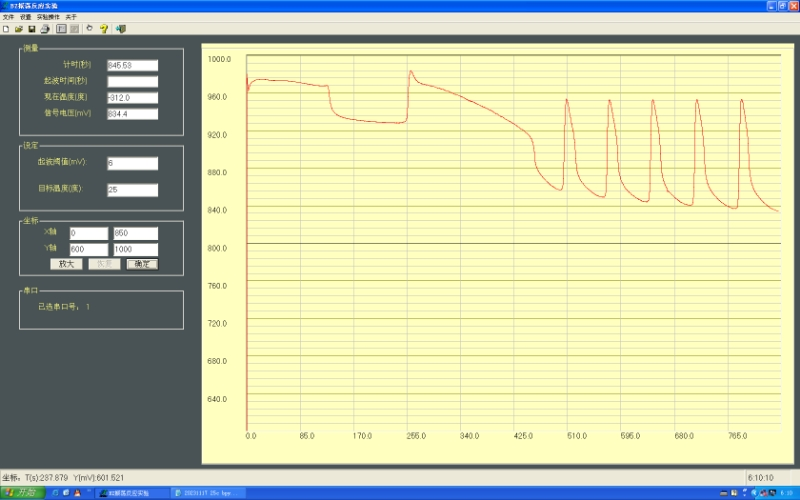
\includegraphics[width=3in]{25.jpg}
        \label{label_for_cross_ref_1}
    }
    \subfigure[30℃的BZ振荡波形]{
		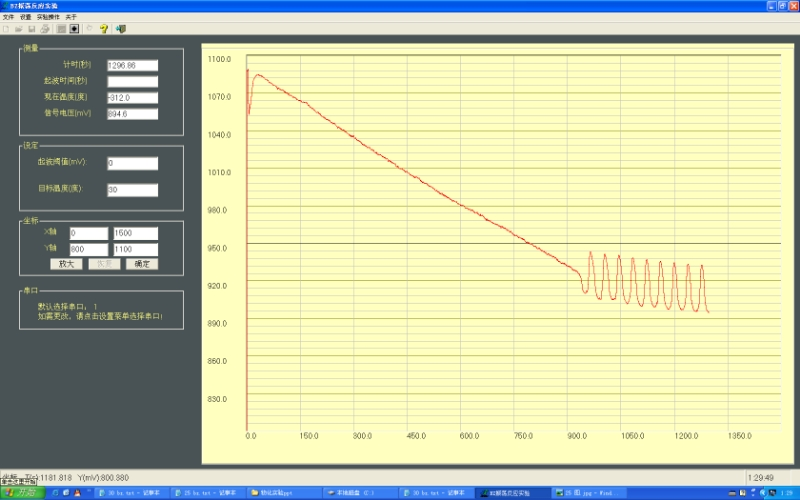
\includegraphics[width=3in]{30.jpg}
        \label{label_for_cross_ref_2}
    }
    \\    %用 \quad 来换行
	    \subfigure[35℃的BZ振荡波形]{
		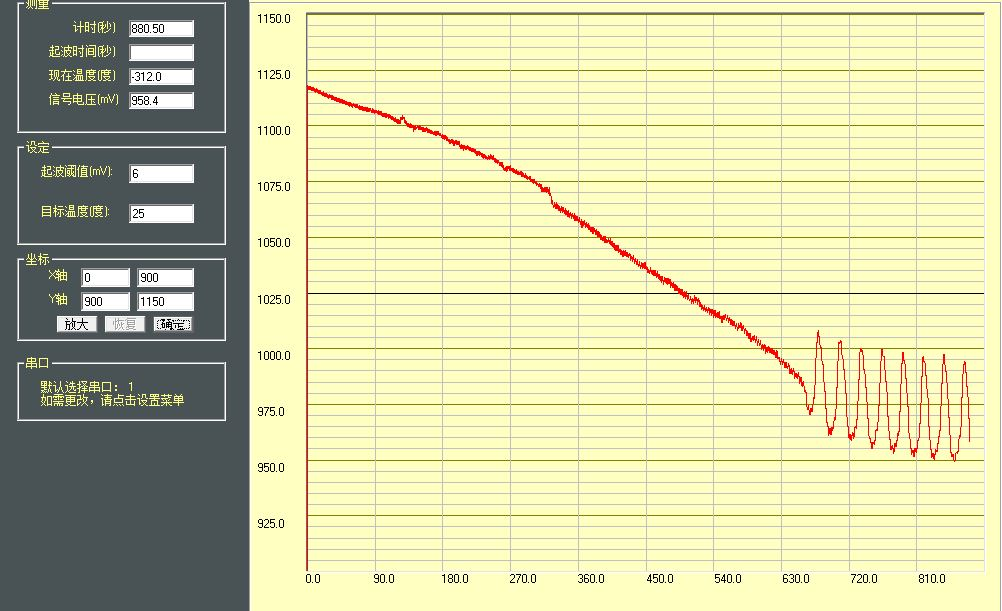
\includegraphics[width=3in]{35.png}
		\label{label_for_cross_ref_1}
	}
	\subfigure[40℃的BZ振荡波形]{
		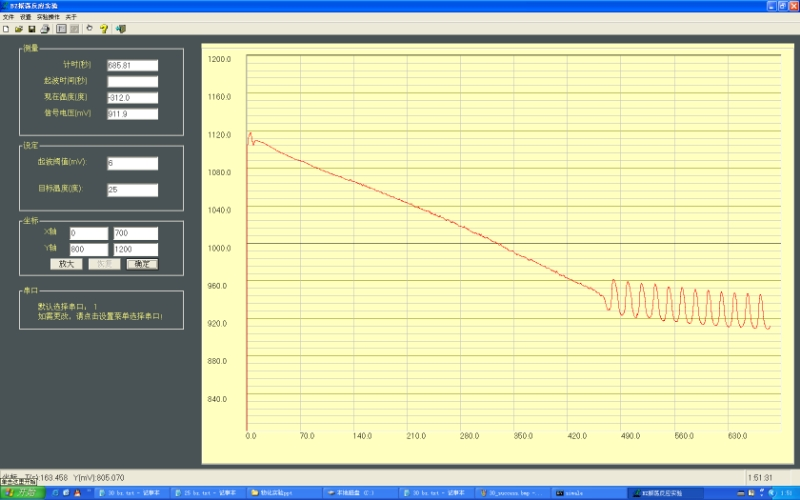
\includegraphics[width=3in]{40.jpg}
		\label{label_for_cross_ref_2}
	}
	\\ 
	    \subfigure[45℃的BZ振荡波形]{
		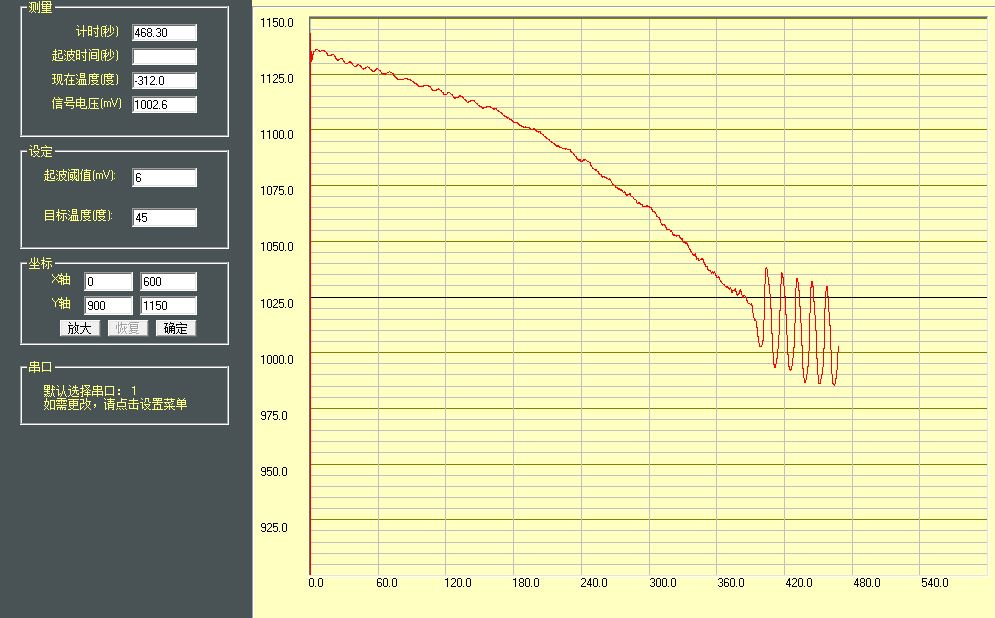
\includegraphics[width=3in]{45.png}
		\label{label_for_cross_ref_1}
	}
\end{figure}
\newpage
\subsubsection{BZ震荡反应数据汇总}
\begin{table}[htp]
	\centering
	\caption{BZ振荡反应数据记录}
	\begin{tabular}{|c|c|c|c|c|c|}
		\hline
		实验温度$t/^{\circ} C$ & $t_{\text{振}}$/s & $t_{\text{诱}}$/s & 1/T(1/K) & ln(1/$t_{\text{诱}}$) & ln(1/$t_{\text{振}}$) \\ \hline
		25      &  781.97  & 61.14 & $3.354\times 10^{-3}$ & -6.666 & -4.113     \\ \hline
		30      &  904.14  & 36.02 & $3.298\times 10^{-3}$ & -6.807 & -3.584         \\ \hline
		35      &  664.74  & 28.26 & $3.245\times 10^{-3}$ & -6.499 & -3.341         \\ \hline
		40      &  476.62  & 16.68 & $3.193\times 10^{-3}$ & -6.167 & -2.814         \\ \hline
		45      &  398.56  & 13.23 & $3.143\times 10^{-3}$ & -5.988 & -2.582         \\ \hline
	\end{tabular}
\end{table}
\subsection{甲酸氧化动力学}
\subsubsection{甲酸氧化动力学实验数据汇总(数据来源于其他小组)}
具体内容见数据分析部分
\newpage
\section{数据分析}
\subsection{BZ振荡反应}
\subsubsection{做出$ln{\frac{1}{t_{\text{诱导}}}}-\frac{1}{T}$图像}
对于拟合图像,观察到 30℃时数据点异常偏低,该温度下的 ln(1/t诱) 值异常偏
小,偏离拟合曲线程度较大。与此同时,拟合结果方差 R平方 = 0.8255,线性并不明确,拟合结果准确性具有明显不足,故选择舍去 30℃ 数据点后重新
进行拟合操作,得到如下结果:
\begin{figure}[H]
	\centering
	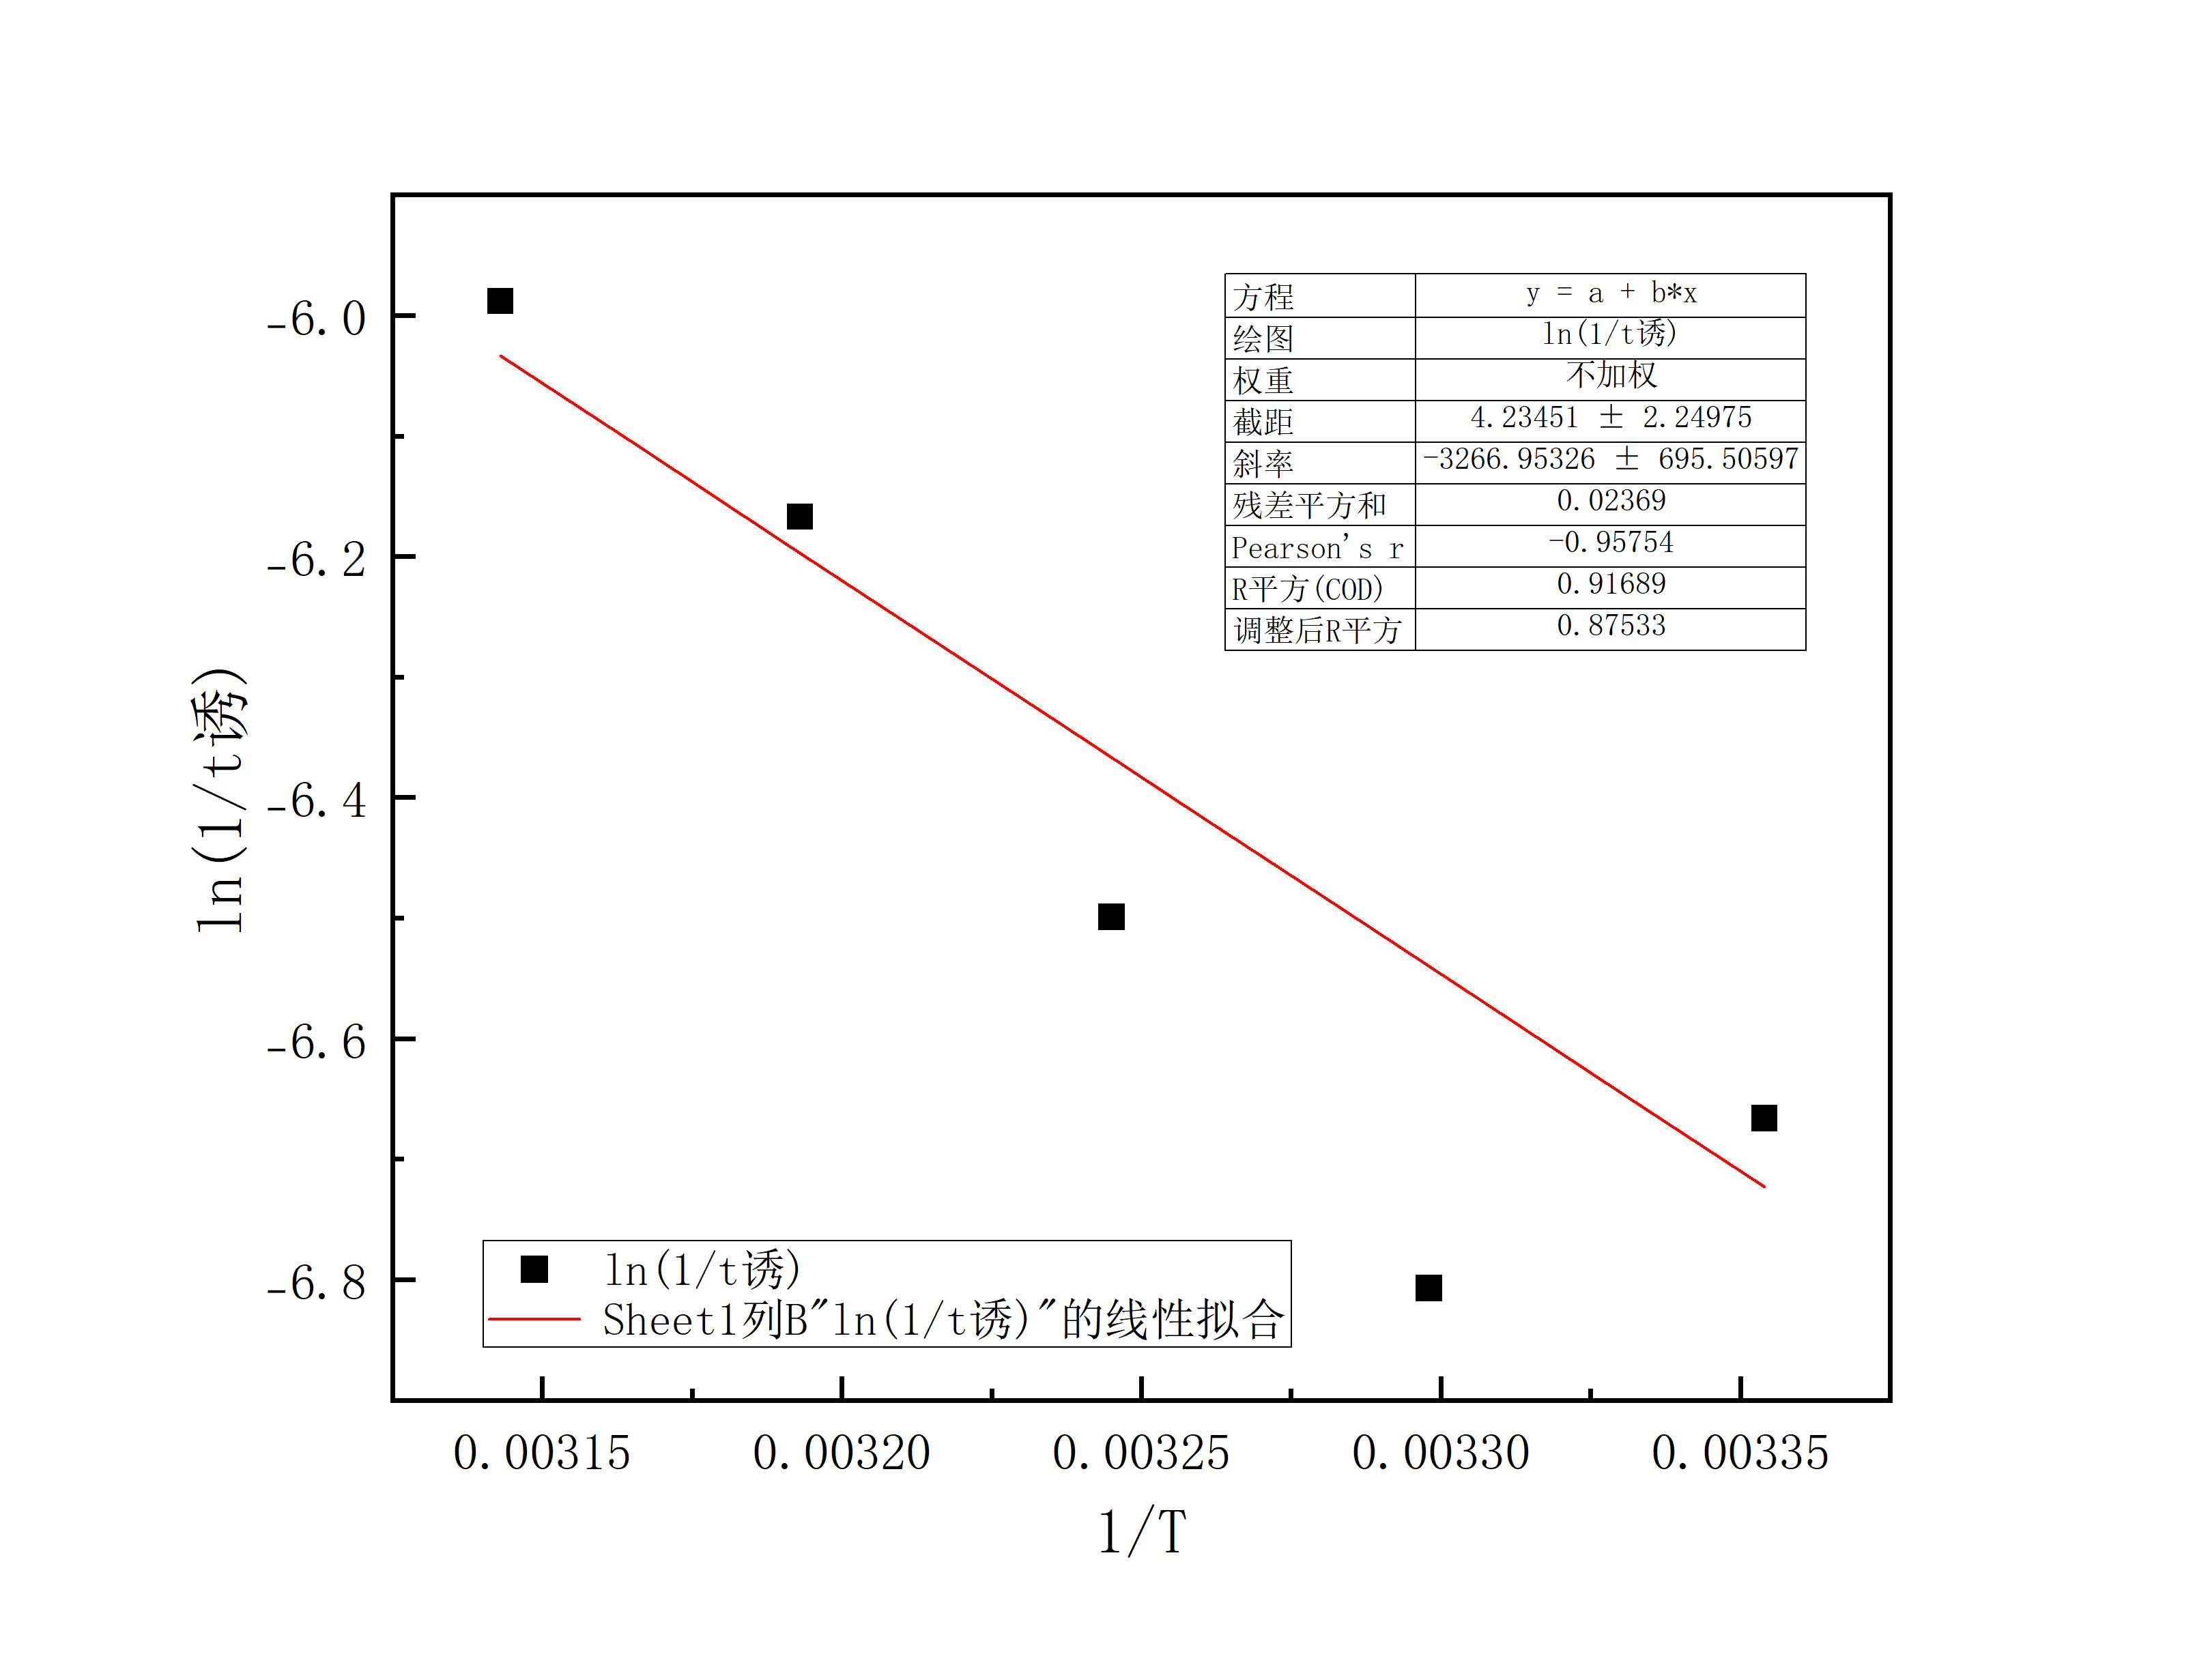
\includegraphics[width=0.6\linewidth]{f1.png}
	\caption{$ln{\frac{1}{t_{\text{诱导}}}}-\frac{1}{T}$图像}
	\label{fig:example}
\end{figure}
根据关系式 
\begin{equation}
	ln(\frac{1}{t}) = -\frac{E}{RT} + C
\end{equation}
可知BZ振荡反应表观诱导活化能
\[
	k = -\frac{E}{R}
\]
\[	
	E_{\text{诱导}} = -kR = 3266.95 \times 8.3145 = 27.163kJ \cdot mol^{-1}
\]

\subsubsection{做出$ln{\frac{1}{t_{\text{振荡}}}}-\frac{1}{T}$图像}
\begin{figure}[H]
	\centering
	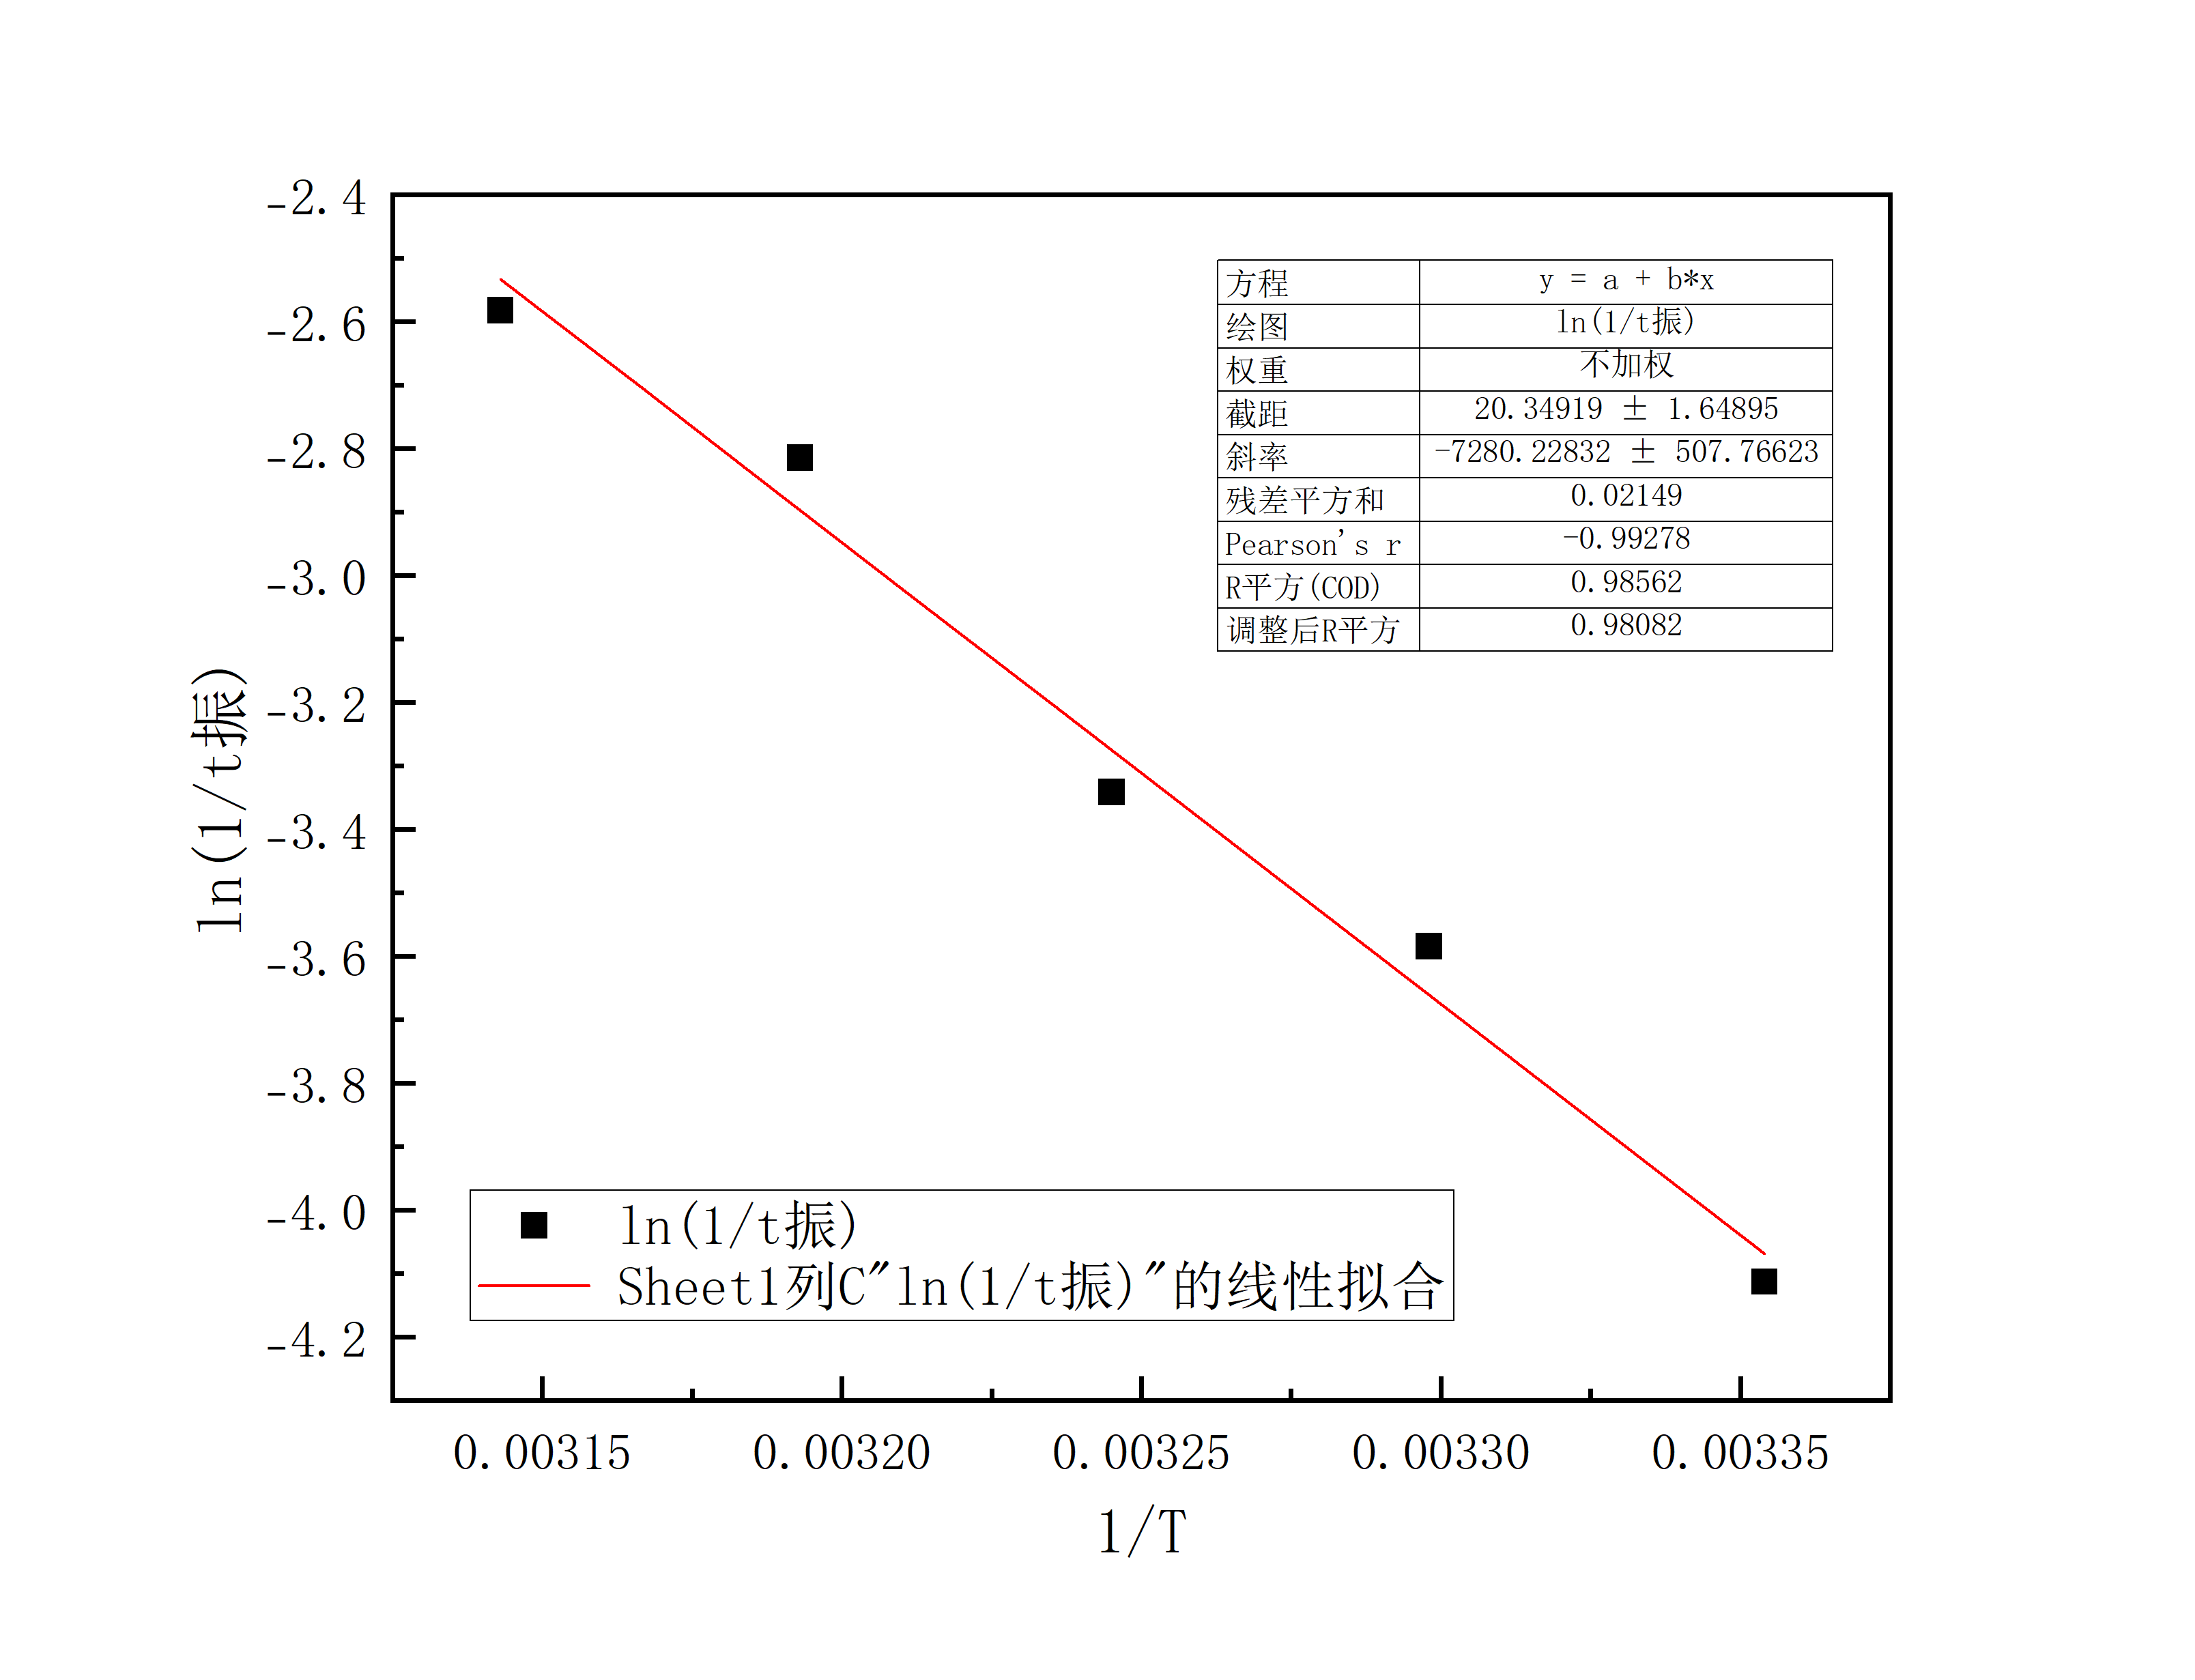
\includegraphics[width=0.6\linewidth]{f2.png}
	\caption{$ln{\frac{1}{t_{\text{振荡}}}}-\frac{1}{T}$图像}
	\label{fig:example}
\end{figure}
拟合结构R平方为0.9856,线性关系可以接受。
根据关系式 
\begin{equation}
	ln(\frac{1}{t}) = -\frac{E}{RT} + C
\end{equation}
可知BZ振荡反应振荡活化能
\[
k = -\frac{E}{R}
\]
\[	
E_{\text{振荡}} = -kR = 7280.22 \times 8.3145 = 60.530kJ \cdot mol^{-1}
\]
\subsection{甲酸氧化动力学}
对五组测定的电动势E分别对t作图,并进行线性拟合,结果如图所示。每组的$R^2$均达到了0.99,线性非常好。由于当反应对溴是一级反应时,即$v=k'[\ce{Br2}]$可推导出
$$
E=Const-(\frac{RT}{2F})k't
$$
由于E-t图确实是直线,可反推出该反应对溴是一级反应,故n=1成立。
\begin{figure}[H]
	\centering
	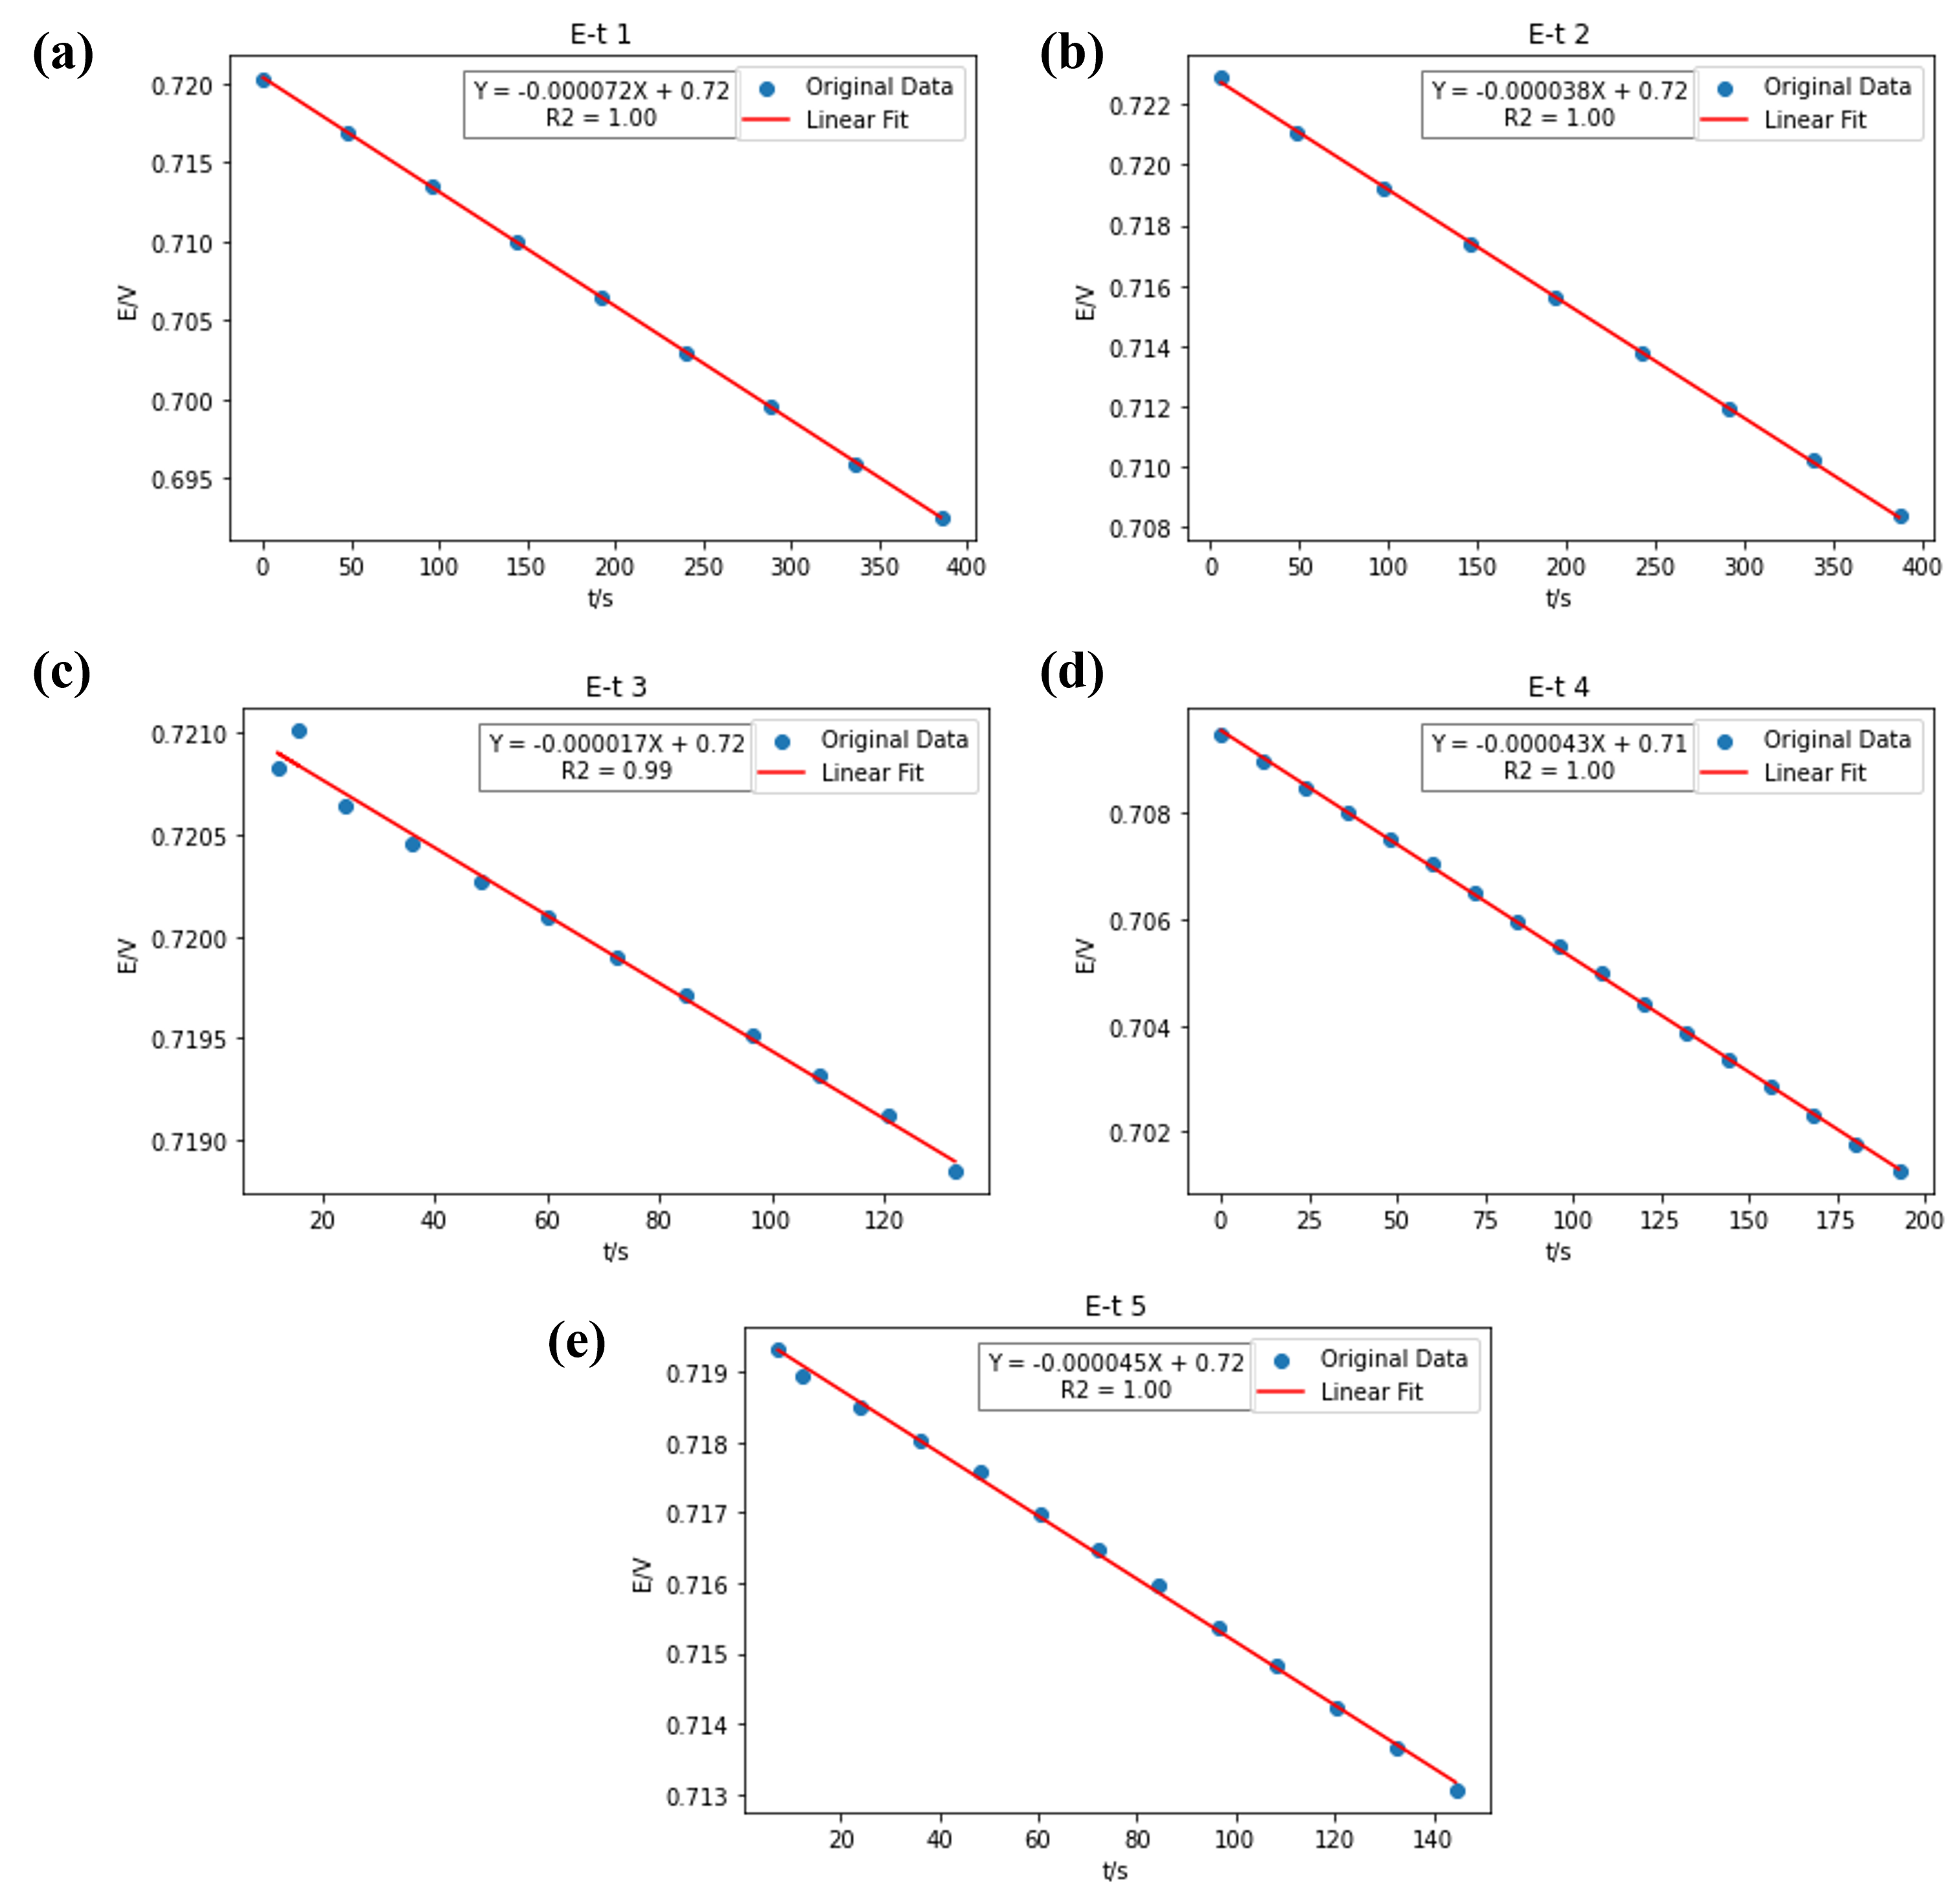
\includegraphics[width = .9\textwidth]{figures/regression3.png}
	\caption{甲酸氧化反应电势-时间曲线}
	\label{fig:BZcurve}
\end{figure}

根据公式
$$
k'=-(\frac{2F}{RT})(\frac{\mathrm{d}E}{\mathrm{d}t})
$$
可求得不同组别的反应速率常数k',结算结果如表\ref{tab:kcal}所示,由于反应是复杂反应,k的单位暂时无法确定。
\begin{table}[H]
	\centering
	\caption{k'计算}
	\label{tab:kcal}
	\begin{tabular}{cccc}
		\hline
		组别 & 斜率        & 温度/K & k'       \\
		\hline
		1  & -0.000072 & 298  & 0.00561 \\
		2  & -0.000038 & 298  & 0.00296  \\
		3  & -0.000017 & 298  & 0.00132 \\
		4  & -0.000043 & 298  & 0.00335  \\
		5  & -0.000045 & 303  & 0.00345 \\
		\hline
	\end{tabular}
\end{table}

根据公式
$$
\frac{k'_1}{k'_2} = \frac{k[HCOOH]_1^m[\ce{H+}]^a[\ce{Br-}]^b}{k[HCOOH]_2^m[\ce{H+}]^a[\ce{Br-}]^b} = \frac{[HCOOH]_1^m}{[HCOOH]_2^m}
$$

可推出
$$
m=\frac{\ln k'_1-\ln k'_2}{\ln[HCOOH]_1-\ln [HCOOH]_2}
$$

同理有
$$
a=\frac{\ln k'_2-\ln k'_3}{\ln[\ce{H+}]_2-\ln [\ce{H+}]_3}
$$

$$
b=\frac{\ln k'_2-\ln k'_4}{\ln[\ce{Br-}]_2-\ln [\ce{Br}]_4}
$$
根据表\ref{tab:HCOOH_real}中的配比,可计算出
\begin{align*}
	[HCOOH]_1=1.14 mol/L \qquad [HCOOH]_2= 0.57 mol/L \\
	[\ce{H+}]_2=0.29 mol/L\qquad [\ce{H+}]_3=0.57mol/L \\
	[\ce{Br-}]_2=0.57mol/L \qquad[\ce{Br}]_4=1.14mol/L
\end{align*}
代入反应级数的表达式可以算出
\begin{align*}
	m=0.92 \approx 1 \\
	a=-1.20 \approx -1\\
	b=0.19 \approx 0
\end{align*}
由公式
$$
k=\frac{k‘}{[HCOOH]^m[\ce{H+}]^a[\ce{Br-}]^b}
$$
代入第一组的k'及浓度数据,计算得到298K下反应速率常数
$$
k_1=1.41 \times 10^{-3}
$$
同理,代入第五组的数据,303K下反应速率常数
$$k_2=1.73\times 10^{-3}
$$
所以298K下甲酸氧化反应的速率方程为
$$
v=-\frac{\mathrm{d [\ce{Br2]}}}{\mathrm{d} t}=1.41\times10^{-3}[HCOOH]^1[\ce{Br2}]^1[\ce{H+}]^{-1}[\ce{Br-}]^0
$$
由阿伦尼乌斯方程
$$
E_{\mathrm{a}}=\frac{R T_1 T_2}{T_2-T_1} \ln \frac{k_2}{k_1}
$$
代入第二组和第五组的温度(298K,303K)和k可以得到反应的活化能
$$
E_a=31141J
$$

\section{结果分析与讨论}
\subsection{BZ振荡反应}
	中国科学技术大学的陈婧(2020)对丙二酸-溴酸钾体系 B-Z 振荡反应进行了研究去,其计算得出
\begin{align*}
	E_{\text{诱}}=47.24 kJ \\
	E_{\text{振}}=59.86 kJ
\end{align*}
	比较自己的计算结果,得出相对误差分别为-42.49\%和1.12\%,后者误差相对较小,而本实验测定的诱导表观活化能具有较大偏差,明显较低。经过分析,我人为可能得原因有以下几点:
\begin{enumerate}
	\item 实验中选取诱导期和振荡期终始点主要依赖人工判断峰值,这种判断可能存在一定误差。建议在读取振荡周期时多读取几个周期的振荡时间数值取平均值,同时取振荡曲线峰值作为读取点,以减小误差。
	\item 反应装置为敞口,反应体系不是封闭体系,反应试剂可能会被空气中物质氧化,影响测定结果。
	若进一步改进反应装置,可以添加橡皮塞,有利于测定精度的提升。
	\item 由于反应试剂被污染,前一个半小时无法得到反应的振荡,最后不同温度下的数据是不同小组共享的,并非是由同一个测量装置测定,可能存在系统误差,改进建议是尽可能使用同一个测量装置进行实验以减小系统误差。
\end{enumerate}
这次实验中最初一个半小时,没有一个小组得到振荡的波形,最后由我们小组通过控制变量的方式,发现了是实验试剂硫酸铈铵被污染,由于BZ振荡反应是一个十分灵敏的反应,一定要保证所有的实际正确配制、没有被污染。这次实验中得到的反思是:使用移液管取溶液时,不同溶液需要不同的移液管,一定要在移液管上做好标签以防实验试剂污染;同时,取试剂时,要将试剂倾倒至烧杯中再使用移液管,这样可以避免容器中所有的试剂都被污染。

\subsection{甲酸氧化动力学}
查阅资料可知甲酸氧化反应活化能的文献值为63580J,因此相对误差
$$
w=\frac{31141-63580}{63580}\times 100 \%=-51\%
$$
	活化能的误差较大,但由于本组数据是共享,因此操作人究竟做了什么导致误差已不得而知,以下仅对实验中可能造成误差的操作及数据计算过程进行评析。

	由于前四组数据用于计算反应级数,结果均接近某个整数,可以认为结果相对准确,因此进行了近似(但不排除反应级数非整数的情况)。用近似为整数后的反应级数和原来计算出的浓度以及k'值计算,本身就会造成一定误差的累积,但不只是这些累积造成-51\%的误差。

	经过分析发现,第五组数据未用来计算前面的反应级数,而第五组是从298K升温到303K,再重复第二组的配比进行实验。根据之前实验的教训(丙酮碘化反应,升温操作出现失误导致活化能计算直接变成负的),升温后如果不再恒温一段时间,很可能反应体系内的温度还未到达303K,造成$k_2$偏小。
	假设体系只升到300.5K,那么计算得出的活化能为60910J,我们认为这可能是造成误差的核心原因。

	不过五组反应的E-t图的线性均非常好,可以认为大部分操作都较为规范,在个别操作细节上还可以改进,实验总体成功。
\section{思考题}
\begin{enumerate}
	\item \textbf{影响诱导期的主要因素有哪些?}
	\begin{enumerate}
		\item 反应温度:温度对化学反应的速率有影响,温度越高,诱导期越短,从实验数据也可以印证这一点。
		\item 反应物的浓度:反应物的浓度也会影响反应的速率,从而影响诱导期。
		\item 反应体系中其他成分:如果在反应初期就加入一定量的溴丙二酸,诱导期会缩短。相反的,如果提高体系中铈的浓度,诱导期则会延长
	\end{enumerate}
	
	
	\item \textbf{实验过程中为什么要尽量保持磁力搅拌的转速相等?}
	在BZ反应中,磁力搅拌器的转速影响了反应物的混合程度。如果转速过慢,反应物混合不均匀,可能会影响反应的进行。保持转速相等可以使振荡反应保持一个相对稳定的状态,否则可能会导致每个振荡周期长度及峰值不同,甚至出现异常点。
	
	
	\item \textbf{如果在振荡开始后加入 KCl 溶液,会发生什么现象,为什么?}
	震荡反应会停止。氯离子会与反应的中间体(HBrO或\ce{HBrO2})反应,干扰了振荡行为。
	
\end{enumerate}
\end{document}